\documentclass[conference,compsoc]{IEEEtran}



% *** CITATION PACKAGES ***
%
\ifCLASSOPTIONcompsoc
  % IEEE Computer Society needs nocompress option
  % requires cite.sty v4.0 or later (November 2003)
  \usepackage[nocompress]{cite}
\else
  % normal IEEE
  \usepackage{cite}
\fi


% *** GRAPHICS RELATED PACKAGES ***
%
\ifCLASSINFOpdf
  % \usepackage[pdftex]{graphicx}
  % declare the path(s) where your graphic files are
  % \graphicspath{{../pdf/}{../jpeg/}}
  % and their extensions so you won't have to specify these with
  % every instance of \includegraphics
  % \DeclareGraphicsExtensions{.pdf,.jpeg,.png}
\else
  % or other class option (dvipsone, dvipdf, if not using dvips). graphicx
  % will default to the driver specified in the system graphics.cfg if no
  % driver is specified.
  % \usepackage[dvips]{graphicx}
  % declare the path(s) where your graphic files are
  % \graphicspath{{../eps/}}
  % and their extensions so you won't have to specify these with
  % every instance of \includegraphics
  % \DeclareGraphicsExtensions{.eps}
\fi



\usepackage{tikz}
\usepackage{graphicx}
\usetikzlibrary{shapes.geometric, arrows}
\tikzstyle{line}=[draw] % here
% correct bad hyphenation here
\hyphenation{op-tical net-works semi-conduc-tor}


\begin{document}
%
% paper title
\title{CSE 591 - Introduction to Deep Learning\\Mini Project 6}


% author names and affiliations
% use a multiple column layout for up to three different
% affiliations
\author{\IEEEauthorblockN{Bijan Fakhri}
\IEEEauthorblockA{School of Computing, Informatics and\\Decision Systems Engineering\\
Arizona State University\\
Tempe, Arizona 85044\\
Email: bfakhri@asu.edu}}

% make the title area
\maketitle

% As a general rule, do not put math, special symbols or citations
% in the abstract
\begin{abstract}

\end{abstract}
 
\IEEEpeerreviewmaketitle


\section{Introduction}


\section{Autoencoders}
Three datasets were tested in these experiments, all derivatives of the MNIST handwritten digit dataset. Below are YANN visualizer outputs of the three datasets. 
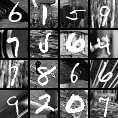
\includegraphics[scale=0.65]{orig}
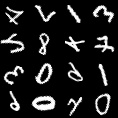
\includegraphics[scale=0.65]{rot}
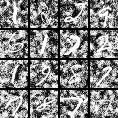
\includegraphics[scale=0.65]{noisy}
From left to right, the datasets above are: the original MNIST dataset, a rotated MNIST dataset, and a noisy MNIST dataset. To measure the generalities, we prejudiced a network using one dataset, recorded its performance, then retrained the softmax layer of that network on another dataset. The generalization performance was then calculated using equation 2. This was done on all possible combinations of the three datasets. 

\section{Generative Adversarial Networks (GAN)}
\section{De-Noising with Autoencoders}

\section{Results}
The results of the experiments are tabulated below. The dataset in the left column corresponding to a cell in the tabel represents the dataset on which the CNN was prejudiced with. The dataset in the top row corresponding to a cell represents the dataset the CNN was tested on (after training the softmax layer). 
 \renewcommand{\arraystretch}{1.2}
 \begin{center}
   \begin{tabular}{ | c || c | c | c | }
     \hline 
     \textbf{MNIST Dataset} & \textbf{Original} & \textbf{Rotated} & \textbf{Noisy} \\ \hline
     \hline
     \textbf{Original} & 1.00 & 0.27 & 0.39 \\ \hline
     \textbf{Rotated} & 0.32 & 1.00 & 0.43 \\ \hline
     \textbf{Noisy}  & 0.39 & 0.28 & 1.00 \\ \hline
   \end{tabular}
 \end{center}
 
From the results it is evident that the rotated version of the MNIST dataset is the most general, sporting an average generality of 0.58, slightly higher than the original and noisy datasets (both at 0.56). Interestingly, the generality of the rotated dataset with respect to the noisy dataset topped the charts at 0.43. 


\section{Conclusion and Discussion}
%
The results unveiled interesting patterns in the generality of the datasets. The generalities with respect to the rotated dataset are interesting because they are the lowest (at 0.27 and 0.28). This could be because the atomic structures learned by the CNN are not rotation invariant. This could explain why the rotated dataset is the most general - prejudicing with it produces rotation invarient filters. It is also interesting to note that the noisy dataset is equally as general as the original. This is not initially expected because noise could act as a regularizer, but, because the CNN is using dropout, it is likely redundant, handing the rotated dataset the crown. 

\nocite{*}
\bibliography{ragav}
%\bibliographystyle{IEEE}
\bibliographystyle{IEEEtran}

%\begin{thebibliography}{1}


%\bibitem{}
%REDO THIS 

%\bibitem{}
%H.~Kopka and P.~W. Daly, \emph{A Guide to \LaTeX}, 3rd~ed.\hskip 1em plus
%  0.5em minus 0.4em\relax Harlow, England: Addison-Wesley, 1999.
  


%\end{thebibliography}

% that's all folks
\end{document}


